\documentclass[11pt]{article}
\usepackage[margin=1in]{geometry}
\usepackage{amsmath,amssymb}
\usepackage{enumitem}
\usepackage{booktabs}
\usepackage{xcolor}
\usepackage{listings}
\usepackage{graphicx}

\setlength{\parindent}{0pt}
\setlength{\parskip}{4pt}
\setlist[enumerate]{label=(\alph*), leftmargin=*, itemsep=8pt}

\lstset{
  language=R,
  basicstyle=\ttfamily\small,
  keywordstyle=\color{blue!70!black},
  commentstyle=\color{gray},
  frame=single,
  rulecolor=\color{gray!60},
  backgroundcolor=\color{gray!6},
  xleftmargin=4pt, xrightmargin=4pt,
  aboveskip=6pt, belowskip=4pt,
  showstringspaces=false,
  columns=fullflexible,
  keepspaces=true
}

% Problem statement style
\newcommand{\prob}[1]{\par\noindent{\color{gray!40!black}\itshape #1}\par\smallskip}

\title{STT 465 -- Homework 2: Single-Parameter Bayesian Models}
\author{Mihir Patel}
\date{Due October 9, 2026}

\begin{document}
\maketitle

%==================================================================
\section*{Question 1: Bernoulli-Beta Posterior \hfill [1 point]}

\prob{A basketball player makes 18 of 25 free throws. Let $X_i \mid \omega \sim \mathrm{Bern}(\omega)$, $i = 1,\dots,25$, where $\omega$ is the player's underlying probability of making a free throw. Assume the prior $\omega \sim \mathrm{Beta}(2,2)$.}

Throughout, let $n = 25$, $s = \sum_{i=1}^{25} x_i = 18$ (makes), and $n - s = 7$ (misses). The prior hyperparameters are $a = b = 2$.

\begin{enumerate}
\item \prob{Write the likelihood function $L(\omega \mid x)$ up to a multiplicative constant that does not depend on $\omega$. [0.2 pt]}
Since the $X_i$ are conditionally independent given $\omega$,
\[
L(\omega \mid x) = \prod_{i=1}^{25} \omega^{x_i}(1-\omega)^{1-x_i}
= \omega^{\sum x_i}(1-\omega)^{\,n-\sum x_i}
= \omega^{18}(1-\omega)^{7}, \qquad 0 \le \omega \le 1.
\]

\item \prob{Use Bayes' theorem to derive the posterior distribution $\pi(\omega \mid x)$. Identify the posterior distribution and its parameters. [0.2 pt]}
The $\mathrm{Beta}(2,2)$ prior density is
\[
\pi(\omega) = \frac{1}{B(2,2)}\,\omega^{2-1}(1-\omega)^{2-1} \propto \omega(1-\omega).
\]
By Bayes' theorem,
\[
\pi(\omega \mid x) = \frac{L(\omega \mid x)\,\pi(\omega)}{\int_0^1 L(\omega \mid x)\,\pi(\omega)\,d\omega}
\;\propto\; \omega^{18}(1-\omega)^{7}\cdot \omega(1-\omega)
= \omega^{19}(1-\omega)^{8}
= \omega^{20-1}(1-\omega)^{9-1}.
\]
This is the kernel of a Beta density, so after normalizing,
\[
\boxed{\;\omega \mid x \sim \mathrm{Beta}(20,\,9)\;}, \qquad
\pi(\omega \mid x) = \frac{1}{B(20,9)}\,\omega^{19}(1-\omega)^{8},\quad 0<\omega<1.
\]
In general, a $\mathrm{Beta}(a,b)$ prior with $s$ successes in $n$ trials gives a $\mathrm{Beta}(a+s,\; b+n-s)$ posterior; here $(2+18,\ 2+7) = (20, 9)$.

\item \prob{Derive the posterior mean $E[\omega \mid x]$ and calculate its numerical value. [0.2 pt]}
For $\omega \sim \mathrm{Beta}(\alpha,\beta)$,
\[
E[\omega] = \int_0^1 \omega \cdot \frac{\omega^{\alpha-1}(1-\omega)^{\beta-1}}{B(\alpha,\beta)}\,d\omega
= \frac{B(\alpha+1,\beta)}{B(\alpha,\beta)}
= \frac{\Gamma(\alpha+1)\,\Gamma(\alpha+\beta)}{\Gamma(\alpha)\,\Gamma(\alpha+\beta+1)}
= \frac{\alpha}{\alpha+\beta},
\]
using $\Gamma(z+1) = z\,\Gamma(z)$. With $\alpha = 20$, $\beta = 9$,
\[
E[\omega \mid x] = \frac{a+s}{a+b+n} = \frac{20}{29} \approx 0.6897.
\]
This lies between the prior mean $2/4 = 0.5$ and the sample proportion $18/25 = 0.72$, closer to the data because $n = 25$ outweighs the prior's effective sample size $a+b = 4$.

\item \prob{Calculate the posterior mode and posterior median. You may use \texttt{qbeta()} for the median. [0.2 pt]}
For $\alpha, \beta > 1$, the Beta mode is found by setting the derivative of the log-density to zero:
\[
\frac{d}{d\omega}\Big[(\alpha-1)\log\omega + (\beta-1)\log(1-\omega)\Big] = \frac{\alpha-1}{\omega} - \frac{\beta-1}{1-\omega} = 0
\;\Longrightarrow\;
\omega_{\text{mode}} = \frac{\alpha-1}{\alpha+\beta-2}.
\]
So
\[
\text{Mode} = \frac{19}{27} \approx 0.7037.
\]
The median has no closed form, so we use the Beta quantile function:
\begin{lstlisting}
qbeta(0.5, shape1 = 20, shape2 = 9)
#> [1] 0.6940678
\end{lstlisting}
\[
\text{Median} \approx 0.6941.
\]
Mean $(0.6897) <$ median $(0.6941) <$ mode $(0.7037)$, consistent with a slightly left-skewed posterior ($\alpha > \beta$).

\item \prob{Use R to calculate $P(\omega > 0.70 \mid x)$. Include the R command you use. [0.2 pt]}
\[
P(\omega > 0.70 \mid x) = 1 - F_{\omega \mid x}(0.70) = \int_{0.70}^{1} \frac{\omega^{19}(1-\omega)^{8}}{B(20,9)}\,d\omega.
\]
\begin{lstlisting}
1 - pbeta(0.70, shape1 = 20, shape2 = 9)
#> [1] 0.4724805

# Equivalent:
pbeta(0.70, shape1 = 20, shape2 = 9, lower.tail = FALSE)
\end{lstlisting}
\[
P(\omega > 0.70 \mid x) \approx 0.4725.
\]
Given the data and prior, there is about a 47\% posterior probability that the player's true free-throw percentage exceeds 70\%.
\end{enumerate}

%==================================================================
\section*{Question 2: Prior Sensitivity and Bayesian Updating \hfill [1 point]}

\prob{Suppose a treatment is effective for 18 of 21 patients. Let $\omega$ denote the probability that the treatment is effective. Consider the two priors
\[
\text{Prior A: } \omega \sim \mathrm{Beta}(1,1), \qquad \text{Prior B: } \omega \sim \mathrm{Beta}(4,\,0.9).
\]}

$18/21$ successes, $\omega$ = probability of the treatment being effective. Posterior $\propto$ likelihood $\times$ prior.

\begin{enumerate}
\item \prob{Derive the posterior distribution under Prior A. [0.2 pt]}
The Beta prior has the form $\omega^{a-1}(1-\omega)^{b-1}$, so
\[
\pi_A(\omega \mid x) \propto \omega^{18}(1-\omega)^{3}\,\omega^{1-1}(1-\omega)^{1-1}
= \omega^{19-1}(1-\omega)^{4-1}
\]
\[
\boxed{\omega \mid x \sim \mathrm{Beta}(19,\,4)}
\]

\item \prob{Derive the posterior distribution under Prior B. [0.2 pt]}
Here the prior is $\omega^{3}(1-\omega)^{-0.1}$, so
\[
\begin{aligned}
\pi_B(\omega \mid x) &\propto \omega^{18}(1-\omega)^{3}\,\omega^{4-1}(1-\omega)^{0.9-1} \\
&= \omega^{21}(1-\omega)^{2.9} \\
&= \omega^{22-1}(1-\omega)^{3.9-1}
\end{aligned}
\]
\[
\boxed{\omega \mid x \sim \mathrm{Beta}(22,\,3.9)}
\]

\item \prob{For a general prior $\omega \sim \mathrm{Beta}(a,b)$, show that the posterior mean can be written as
\[
E[\omega \mid x] = \frac{a+b}{a+b+n}\cdot\frac{a}{a+b} + \frac{n}{a+b+n}\cdot\frac{x}{n}.
\]
Explain what the two terms represent. [0.2 pt]}
$\omega \mid x \sim \mathrm{Beta}(a+x,\ b+n-x)$, and a $\mathrm{Beta}(\alpha,\beta)$ has mean $\dfrac{\alpha}{\alpha+\beta}$. So
\[
\begin{aligned}
E[\omega \mid x] &= \frac{a+x}{(a+x)+(b+n-x)} = \frac{a+x}{a+b+n}
= \frac{a}{a+b+n} + \frac{x}{a+b+n} \\
&= \boxed{\frac{a+b}{a+b+n}\cdot\frac{a}{a+b} + \frac{n}{a+b+n}\cdot\frac{x}{n}}
\end{aligned}
\]
$\dfrac{a}{a+b}$ is the prior mean, weighted by $\dfrac{a+b}{a+b+n}$. $\dfrac{x}{n}$ is the observed success proportion, weighted by $\dfrac{n}{a+b+n}$.

\item \prob{Compute the posterior mean under Priors A and B. Briefly explain why the two answers differ. [0.2 pt]}
$E[\omega \mid x] = \dfrac{\alpha}{\alpha+\beta}$.

Prior A, $\mathrm{Beta}(19,4)$:
\[
E[\omega \mid x] = \frac{19}{19+4} = \frac{19}{23} \approx \boxed{0.8261}
\]
Prior B, $\mathrm{Beta}(22,3.9)$:
\[
E[\omega \mid x] = \frac{22}{25.9} \approx \boxed{0.8494}
\]
They differ because the priors express different beliefs. Prior A has a lower mean, which means Prior A will pull the posterior mean down, below the observed success proportion.

\item \prob{Use R to plot the two posterior densities on the same graph. Add a vertical line at the sample proportion $\tilde{\omega} = 18/21$. Briefly describe what the plot shows. [0.2 pt]}
\begin{lstlisting}
# Plot posterior densities
curve(dbeta(x, shape1 = 19, shape2 = 4),
      from = 0, to = 1,
      col = "blue", lwd = 2, ylim = c(0, 6),
      xlab = expression(omega),
      ylab = "Posterior density",
      main = "Posterior Distributions: Priors A and B")

curve(dbeta(x, shape1 = 22, shape2 = 3.9),
      add = TRUE, col = "red", lwd = 2)

# Mark the observed success proportion
abline(v = 18 / 21, col = "black", lty = 2, lwd = 2)

legend("topleft",
       legend = c("Prior A: Beta(19, 4)",
                  "Prior B: Beta(22, 3.9)",
                  "Sample proportion: 18/21"),
       col = c("blue", "red", "black"),
       lty = c(1, 1, 2), lwd = 2, bty = "n")
\end{lstlisting}
\begin{center}
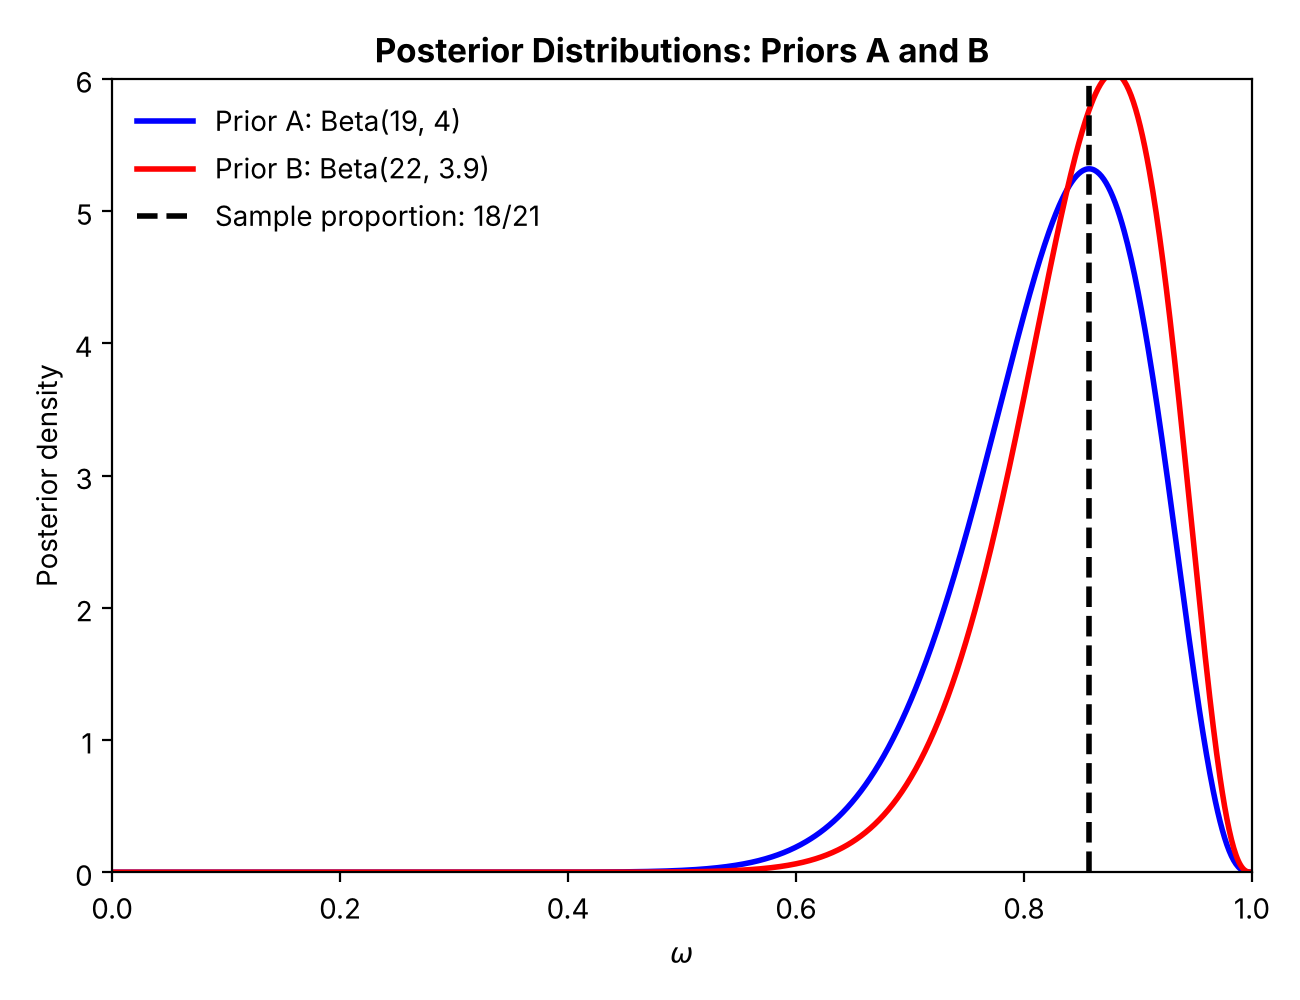
\includegraphics[width=0.65\linewidth]{q2e_plot.png}
\end{center}
Both posteriors are concentrated near the sample proportion $18/21 \approx 0.857$ and overlap heavily. The Prior B posterior is shifted slightly to the right and is a little more peaked, while the Prior A posterior sits slightly lower. With 21 observations, the data dominate and the choice of prior has only a small effect.
\end{enumerate}

%==================================================================
\section*{Question 3: Credible Intervals and HPDI \hfill [1 point]}

\prob{Suppose that after observing data, the posterior distribution is $\omega \mid x \sim \mathrm{Beta}(22, 4)$.}

\begin{enumerate}
\item \prob{Write the R commands needed to calculate the 95\% equal-tailed credible interval \[\big[F^{-1}_{\omega\mid x}(0.025),\ F^{-1}_{\omega\mid x}(0.975)\big].\] Report the numerical interval. [0.2 pt]}
\begin{lstlisting}
# 95% equal-tailed credible interval
equal_tailed <- qbeta(c(0.025, 0.975), shape1 = 22, shape2 = 4)
print(equal_tailed)
\end{lstlisting}
\[
(0.68781,\ 0.95462)
\]

\item \prob{Explain in one or two sentences the Bayesian interpretation of this 95\% credible interval. [0.2 pt]}
Given the observed data and the assumed model and prior, the posterior probability that $\omega$ lies between $0.68781$ and $0.95462$ is 95\%.

\item \prob{Generate 10{,}000 posterior samples using \texttt{set.seed(1)} and \texttt{omega\_post <- rbeta(10000, shape1 = 22, shape2 = 4)}. Use the \texttt{HDInterval} package to estimate the 95\% HPDI. [0.2 pt]}
\begin{lstlisting}
# Install HDInterval automatically if it isn't already installed
if (!requireNamespace("HDInterval", quietly = TRUE)) {
  install.packages("HDInterval", repos = "https://cloud.r-project.org")
}

# 95% highest posterior density interval (HPDI)
set.seed(1)
omega_post <- rbeta(10000, shape1 = 22, shape2 = 4)

hpdi <- HDInterval::hdi(omega_post, credMass = 0.95)
print(hpdi)
\end{lstlisting}
\[
[0.70898,\ 0.96719]
\]

\item \prob{Compare the equal-tailed credible interval and the HPDI. Which one is shorter? [0.2 pt]}
The shorter one is the HPDI, which has a smaller width.

\item \prob{Explain why the two intervals need not be identical for a skewed posterior distribution. [0.2 pt]}
$\mathrm{Beta}(22,4)$ is left-skewed, with a longer tail toward smaller values. Equal-tailed intervals put equal probability in both tails, but the HPDI prioritizes the highest-density values, so the HPDI shifts toward larger values.
\end{enumerate}

%==================================================================
\section*{Question 4: Comparing Two Population Proportions \hfill [1 point]}

\prob{A study of births reports that among 980 births in one group, 437 were female. In a second group, among 820 births, 398 were female. Let $\omega_x$ = female birth proportion in group 1 and $\omega_y$ = female birth proportion in group 2. Assume independent priors $\omega_x \sim \mathrm{Beta}(1,1)$, $\omega_y \sim \mathrm{Beta}(1,1)$.}

Group 1: $437/980$ ($\omega_x$); group 2: $398/820$ ($\omega_y$). In general, a $\mathrm{Beta}(a,b)$ prior gives a $\mathrm{Beta}(a+k,\ b+n-k)$ posterior.

\begin{enumerate}
\item \prob{Derive the posterior distributions of $\omega_x$ and $\omega_y$. [0.2 pt]}
\[
L(\omega_x \mid x) = \binom{980}{437}\omega_x^{437}(1-\omega_x)^{543} \propto \omega_x^{437}(1-\omega_x)^{543}
\]
\[
\pi(\omega_x) \propto \omega_x^{1-1}(1-\omega_x)^{1-1} = 1
\]
\[
\pi(\omega_x \mid x) \propto \omega_x^{437}(1-\omega_x)^{543}
\]
\[
\alpha - 1 = 437 \Rightarrow \alpha = 438, \qquad \beta - 1 = 543 \Rightarrow \beta = 544
\]
\[
\boxed{\omega_x \mid x \sim \mathrm{Beta}(438,\,544)}
\]
Similarly,
\[
\pi(\omega_y \mid y) \propto \omega_y^{398}(1-\omega_y)^{422}\,\omega_y^{0}(1-\omega_y)^{0}
\]
\[
\alpha - 1 = 398 \Rightarrow \alpha = 399, \qquad \beta - 1 = 422 \Rightarrow \beta = 423
\]
\[
\boxed{\omega_y \mid y \sim \mathrm{Beta}(399,\,423)}
\]

\item \prob{Calculate the posterior means $E[\omega_x \mid x]$ and $E[\omega_y \mid y]$. [0.2 pt]}
\[
E[\omega_x \mid x] = \frac{\alpha}{\alpha+\beta} = \frac{438}{438+544} \approx \boxed{0.4460}
\]
\[
E[\omega_y \mid y] = \frac{399}{822} \approx \boxed{0.4854}
\]

\item \prob{Use the posterior simulation idea to estimate $P(\omega_x < \omega_y \mid x, y)$. Complete the missing parts of the R code. [0.2 pt]}
\begin{lstlisting}
set.seed(1)
U <- 10000

omega_x <- rbeta(
  U,
  shape1 = 438,
  shape2 = 544
)

omega_y <- rbeta(
  U,
  shape1 = 399,
  shape2 = 423
)

print(mean(omega_x < omega_y))
\end{lstlisting}
\[
P(\omega_x < \omega_y \mid x, y) \approx 0.953
\]

\item \prob{Explain in words what the probability $P(\omega_x < \omega_y \mid x, y)$ means. [0.2 pt]}
It is the posterior probability that the female birth proportion for group 2 is greater than the female birth proportion for group 1, given $x$ and $y$.

\item \prob{A frequentist analysis uses \texttt{prop.test(c(437, 398), c(980, 820),} \texttt{alternative = "less")}. Briefly explain the difference between the posterior probability in part (c) and the frequentist p-value. [0.2 pt]}
\begin{lstlisting}
# (e) A frequentist analysis uses
print(prop.test(
  c(437, 398),
  c(980, 820),
  alternative = "less"
))
\end{lstlisting}
The test gives $X^2 = 2.6371$, $\text{df} = 1$, and a p-value of $0.0522$.

The difference is that the p-value only gives the probability, assuming the two population proportions are equal, of an observed difference at least as extreme as the one observed in the direction of group 1 having a lower proportion. Part (c), however, is the probability that group 1's true female birth rate is lower than group 2's, given the observed data and prior.
\end{enumerate}

%==================================================================
\section*{Question 5: Poisson-Gamma Model and Prediction \hfill [1 point]}

\prob{Suppose the number of customer complaints received by a company on day $i$ satisfies $X_i \mid \lambda \sim \mathrm{Poi}(\lambda)$, $i = 1,\dots,n$. Over 20 days, a total of 54 complaints are observed: $n = 20$, $\sum_{i=1}^{20} x_i = 54$. Assume the Gamma prior $\lambda \sim \mathrm{Ga}(a = 2,\ b = 1)$, where $a$ is the shape and $b$ is the rate.}

$n = 20$, $\sum_{i=1}^{20} x_i = 54$, $\lambda \sim \mathrm{Ga}(a=2,\ b=1)$. The posterior parameters are $a + \sum_i x_i$ and $b + n$.

\begin{enumerate}
\item \prob{Show that the likelihood function has the form $L(\lambda \mid x) \propto \lambda^{\sum_i x_i}\exp(-n\lambda)$. [0.2 pt]}
\[
L(\lambda \mid x) = \prod_i \frac{\lambda^{x_i}e^{-\lambda}}{x_i!} = \frac{\lambda^{\sum x_i}e^{-n\lambda}}{\prod_i x_i!}
\]
\[
\boxed{L(\lambda \mid x) \propto \lambda^{54}e^{-20\lambda}}
\]

\item \prob{Derive the posterior distribution of $\lambda$ and identify its parameters. [0.2 pt]}
\[
\pi(\lambda) \propto \lambda^{a-1}e^{-b\lambda} = \lambda^{1}e^{-\lambda}
\]
\[
\pi(\lambda \mid x) \propto \lambda^{54+2-1}e^{-(20+1)\lambda}
\]
\[
\boxed{\lambda \mid x \sim \mathrm{Gamma}(56,\,21)}
\]

\item \prob{Calculate the posterior mean $E[\lambda \mid x]$ and a 95\% equal-tailed credible interval using \texttt{qgamma()}. [0.2 pt]}
\begin{lstlisting}
56 / 21
qgamma(c(0.025, 0.975), shape = 56, rate = 21)
\end{lstlisting}
\[
\boxed{E[\lambda \mid x] = \frac{56}{21} \approx 2.667}
\qquad
\boxed{[2.01437,\ 3.40905]}
\]

\item \prob{Derive the posterior predictive mean for the number of complaints on a future day, $E[X_f \mid x]$. Explain why it is equal to $E[\lambda \mid x]$. [0.2 pt]}
We know $X_f \mid \lambda \sim \mathrm{Poisson}(\lambda)$, so $E[X_f \mid \lambda] = \lambda$.
\[
E[X_f \mid x] = E_{\lambda \mid x}\big[E(X_f \mid \lambda, x)\big] = E_{\lambda \mid x}[\lambda]
\]
\[
\boxed{E[X_f \mid x] = \frac{56}{21} \approx 2.667}
\]
Given $\lambda$, future counts follow a Poisson distribution with a mean of $\lambda$, and we average the conditional Poisson mean over the posterior distribution of $\lambda$.

\item \prob{Use posterior simulation to estimate $P(X_f \ge 4 \mid x)$. Report your estimate and explain what it means. [0.2 pt]}
\begin{lstlisting}
set.seed(1)
U <- 10000

lambda_post <- rgamma(
  U,
  shape = 56,
  rate = 21
)

x_future <- rpois(U, lambda = lambda_post)
mean(x_future >= 4)
\end{lstlisting}
\[
\hat{P}(X_f \ge 4 \mid x) = 0.283
\]
Given the observed data, there is approximately a 28.3\% chance of receiving at least 4 complaints on a future day.
\end{enumerate}

\end{document}
